\begin{surferPage}{케일리의 삼차식}
  이 $3$차 곡면은 총 $4$개의 이중 원뿔 형태의 특이점을 가지고 있습니다. 이 식은 $19$세기에 삼차식에 관련해 많은 연구를 한 영국의 수학자 아서 케일리의 이름을 따서 케일리의 $3$차식 이라고 합니다.
    
Ludwig Schl\"afli는 1983년에 처음으로 곡면이 가질 수 있는 특이점을 바탕으로 한 체계적인 방법으로 곡면들을 분류하였습니다. 그의 논문을 보면 왜 $3$차식이 $5$개 이상의 특이점을 가질 수 없는가 설명되어 있습니다. 이말인 즉슨 $\mu(3)=4$ 라는 것입니다. 
 
    
1900년즈음 펠릭스 클라인이라는 독일의 수학자는 $3$차 곡면이 가질 수 있는 모양에 대해 연구하였습니다. 그는 케일리 삼차식으로부터의 변형을 이용하여 이 질문에 대한 답을 내놓았습니다. 이중 원뿔의 특이점을 확장 그리고 끊고 혹은 합치면서 $3$차 곡면이 가질 수 있는 모든 모양을 찾아냈습니다. 다음은 그 중 몇 가지 입니다. 
    \vspace{0.3cm}
     \begin{center}
      \vspace{-0.2cm}
      \begin{tabular}{@{}c@{\ }c@{\ }c@{\ }c@{}}
        \begin{tabular}{@{}c@{}}
          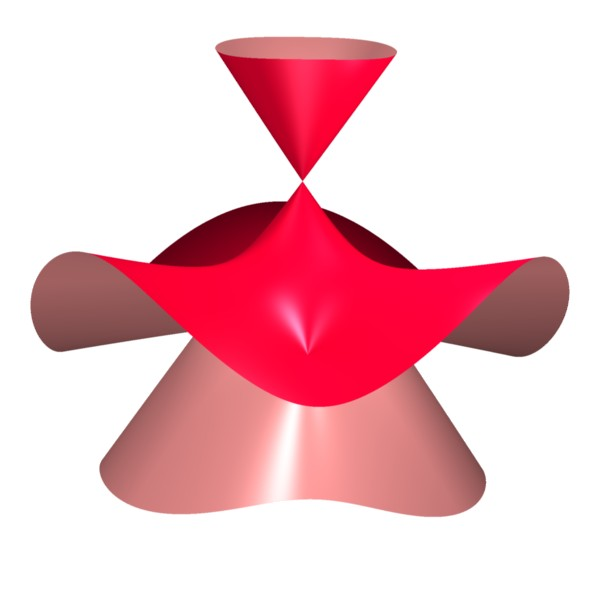
\includegraphics[width=1.35cm]{./../../common/images/cayley_cubic_0}
        \end{tabular}
        &
        \begin{tabular}{@{}c@{}}
          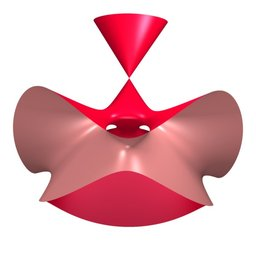
\includegraphics[width=1.35cm]{./../../common/images/cayley_cubic_1}
        \end{tabular}
        &
        \begin{tabular}{@{}c@{}}
          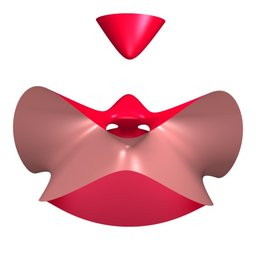
\includegraphics[width=1.35cm]{./../../common/images/cayley_cubic_2}
        \end{tabular}
        &
        \begin{tabular}{@{}c@{}}
          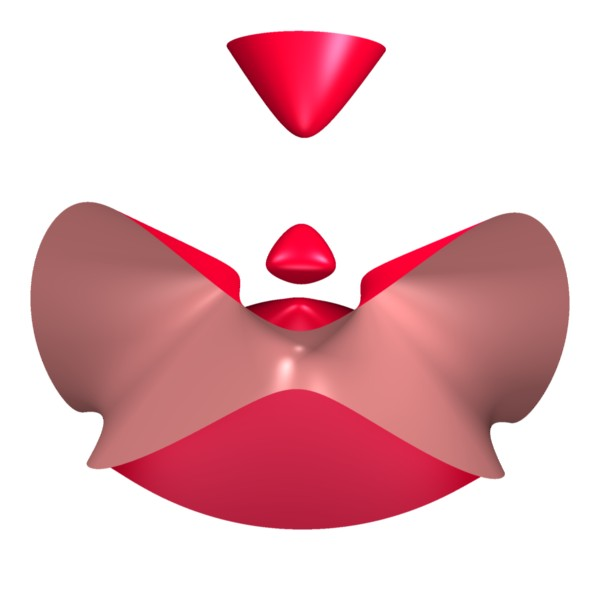
\includegraphics[width=1.35cm]{./../../common/images/cayley_cubic_3}
        \end{tabular}
      \end{tabular}
    \end{center}
\end{surferPage}
